documentclass[letter,11pt,oneside,spanish]{article}
% \usepackage[utf8x]{inputenc}
\usepackage[latin1]{inputenc}
\usepackage[spanish]{babel}
\usepackage{graphicx}
\usepackage{float}
\usepackage{hyperref}
\usepackage{anysize}
\renewcommand{\rmdefault}{phv} % Arial
\renewcommand{\sfdefault}{phv} % Arial

\marginsize{2.5cm}{2.5cm}{2.5cm}{2.5cm}
\renewcommand{\baselinestretch}{1.5}


%opening
\title{\textbf{Teor\'ia del aprendizaje social aplicada a los nuevos paradigmas de conectivismo digital}}
\author{Carlos Caballero, Antonio Mamani\\
        Documento de Investigaci\'on\\
        Universidad Mayor de San Sim\'on\\
	\{cijkb.j,antonio.mq\}@gmail.com\\}
\date{}
\begin{document}

% \maketitle
\newpage
\thispagestyle{empty}
\begin{flushright}
\textit{``Si ayudo a una sola persona a tener esperanza, no habr\'e vivido en vano.''}\\
\textsc{Martin Luther King}
\end{flushright}


\newpage
\section{Introducci\'on}
Con la acelerada reducci\'on de las brechas de accesibilidad digital y la voraz saturaci\'on de las tecnolog\'ias m\'oviles en el
uso cotidiano, el comportamiento de las sociedades con respecto a su cultura tecnol\'ogica se ha convertido en algo inherente;
creando inmejorables oportunidades en el \'ambito educativo. Aplicando las reglas b\'asicas del aprendizaje social se definen 
cuatro etapas a tomar en cuenta: contacto cercano, imitaci\'on de los superiores, comprensi\'on de los conceptos y comportamiento
del modelo a seguir. La sociedad boliviana en el ultimo siglo se ha retrasado en la evoluci\'on social respecto a otros pa\'ises
lo cual ha imposibilitado la construcci\'on de conocimiento propio e innovador que influya en la sociedad. Bas\'andonos en estos
emergentes problemas y la prioritaria necesidad de solucionarlos, se ha construido una red social; base en la cual se 
experimentan las teor\'ias sociol\'ogicas antes mencionadas, con el prop\'osito de crear una herramienta de apoyo en la educaci\'on
superior y secundaria; de esta manera conseguir adecuar los paradigmas de aprendizaje a un modelo mas localizado, donde 
intervengan todas las personas aficionadas al \'area de estudio y as\'i puedan trabajar en un modelo libre de jerarqu\'ias, mas 
ameno y menos formal.
Se plantea la hip\'otesis que la sociedad nacional esta sumida en una especie de letargo, haciendo de la mayor\'ia de sus 
ciudadanos seres de comportamiento individualista y conformista, pero a\'un as\'i podr\'ian despertar a un salto tecnol\'ogico, 
basado en una abierta actitud a compartir, transferir y construir conocimiento de modo irrestricto.

\section{Marco Te\'orico}

\subsection{Aprendizaje}
El aprendizaje \footnote{Aprendizaje definido en wikipededia \url{http://es.wikipedia.org/wiki/Aprendizaje}} es el proceso a
trav\'es del cual se adquieren o modifican habilidades, destrezas, conocimientos, conductas o valores como resultado del 
estudio, la experiencia, la instrucci\'on, el razonamiento y la observaci\'on. Este proceso puede ser
analizado desde distintas perspectivas, por lo que existen distintas teor\'ias del aprendizaje.\\

De todas las teor\'ias de aprendizaje que existen, el conectivismo digital es la evoluci\'on de estas teor\'ias como se
muestra en la figura \ref{learning} \footnote{El gr\'afico fue extra\'ido del blog de Andres Schuschny. \cite{as}}.

\begin{figure}[h]
\centering
 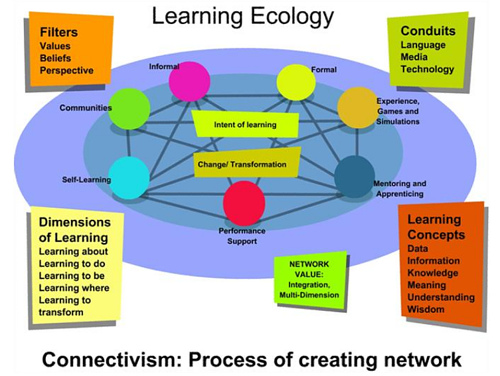
\includegraphics[scale=0.5]{graphics/learning}
 \caption{Ecolog\'ia del aprendizaje.}
 \label{learning}
\end{figure}



\subsection{Conectivismo digital}
El Conectivismo fue presentado como una teor\'ia del aprendizaje basado en la premisa de que el conocimiento existe en el 
mundo en lugar de encontrarse en la cabeza de un individuo. El Conectivismo propone una perspectiva similar a la teor\'ia 
de la actividad(AT) \footnote{Wikipedia: La Teor\'ia de la actividad es una meta-teor\'ia, paradigma, o marco de estudio no 
psicol\'ogico, con ra\'ices dadas por la psicolog\'ia hist\'orica-cultural del psic\'ologo sovi\'etico Lev Vygotsky.} 
de Vygotsky, ya que se refiere al conocimiento que existe dentro de los sistemas que se accede a trav\'es de las
personas que participan en las actividades.\\
El art\'iculo ``Conectivismo: una teor\'ia del aprendizaje para la era digital",propuesto por George Siemens 
\cite{Conetivismo} define que 
%  indica la especial importancia que se da a la tecnolog\'ia de efecto 
% tiene sobre c\'omo vive la gente, c\'omo se comunican, y c\'omo aprenden.\\
% La teor\'ia del conectivismo es propuesto por George Siemens 
el conectivismo es la integraci\'on de principios explorados por las teor\'ias de caos, redes, complejidad y auto-organizaci\'on.
El aprendizaje es un proceso que ocurre al interior de ambientes difusos de elementos centrales cambiantes - que no est\'an 
por completo bajo control del individuo. El aprendizaje (definido como conocimiento aplicable) puede residir fuera de 
nosotros (al interior de una organizaci\'on o una base de datos), est\'a enfocado en conectar conjuntos de informaci\'on 
especializada, y las conexiones que nos permiten aprender m\'as tienen mayor importancia que nuestro estado actual de 
conocimiento.\\

El conectivismo es orientado por la comprensi\'on que las decisiones est\'an basadas en principios que cambian r\'apidamente. 
Continuamente se est\'a adquiriendo nueva informaci\'on. La habilidad de realizar distinciones entre la informaci\'on 
importante y no importante resulta vital. Tambi\'en es cr\'itica la habilidad de reconocer cu\'ando una nueva informaci\'on
altera un entorno basado en las decisiones tomadas anteriormente.\\

Principios del conectivismo:
\begin{itemize}
 \item El aprendizaje y el conocimiento dependen de la diversidad de opiniones. 
 \item El aprendizaje es un proceso de conectar nodos o fuentes de informaci\'on especializados.
 \item El aprendizaje puede residir en dispositivos no humanos. 
 \item La capacidad de saber m\'as es m\'as cr\'itica que aquello que se sabe en un momento dado. 
 \item La alimentaci\'on y mantenimiento de las conexiones es necesaria para facilitar el aprendizaje continuo. 
 \item La habilidad de ver conexiones entre \'areas, ideas y conceptos es una habilidad clave. 
 \item La actualizaci\'on (conocimiento preciso y actual) es la intenci\'on de todas las actividades conectivistas de
       aprendizaje. 
 \item La toma de decisiones es, en s\'i misma, un proceso de aprendizaje. El acto de escoger qu\'e aprender y el significado
       de la informaci\'on que se recibe, es visto a trav\'es del lente de una realidad cambiante. Una decisi\'on correcta 
       hoy, puede estar equivocada ma\~nana debido a alteraciones en el entorno informativo que afecta la decisi\'on. 
\end{itemize}

conectivismo tambi\'en contempla los retos que muchas corporaciones enfrentan en actividades de gesti\'on del conocimiento. 
El conocimiento que reside en una base de datos debe estar conectado con las personas precisas en el contexto adecuado para
que pueda ser clasificado como aprendizaje. El conductismo, el cognitivismo y el constructivismo no tratan de referirse a 
los retos del conocimiento y la transferencia organizacional.
El flujo de informaci\'on dentro de una organizaci\'on es un elemento importante de la efectividad organizacional.\\

En una econom\'ia del conocimiento, el flujo de informaci\'on es el equivalente de la tuber\'ia de petr\'oleo en la sociedad 
industrial. Crear, preservar y utilizar el flujo de informaci\'on deber\'ia ser una actividad organizacional clave. 
El flujo de informaci\'on puede ser comparado con un r\'io que fluye a trav\'es de la ecolog\'ia de una organizaci\'on. 
En ciertas \'areas, el r\'io se estanca y en otras declina. La salud de la ecolog\'ia de aprendizaje de una organizaci\'on depende
del cuidado efectivo del flujo informativo. El an\'alisis de redes sociales es un elemento adicional para comprender los 
modelos de aprendizaje de la era digital. Art Kleiner (2002) explora la ''teor\'ia cu\'antica de la confianza'' de Karen 
Stephenson, la cual ``explica no s\'olo c\'omo reconocer la capacidad cognitiva colectiva de una organizaci\'on, sino c\'omo 
cultivarla e incrementarla''. Al interior de las redes sociales, los hubs \footnote{Esta es la palabra utilizada en el 
original, que no tiene una traducci\'on directa al espa\~nol. Un hub es el punto central en el que se concentran rutas o 
tr\'afico para ser redistribuidas o redirigidas; en telecomunicaciones, un hub es un ``concentrador'' que cumple una funci\'on 
similar en una red de computadores: concentrar y redistribuir el tr\'afico de red.} son personas bien conectadas, capaces 
de promover y mantener el flujo de informaci\'on.\\

Su interdependencia redunda en un flujo informativo efectivo, permitiendo la comprensi\'on personal del estado de actividades
desde el punto de vista organizacional. 
\subsection{Teor\'ia del aprendizaje social}
% La teor\'ia del aprendizaje social de Bandura, que propone que las personas aprenden a trav\'es del contacto.
La Teor\'ia del aprendizaje social se deriva de la obra de Albert Bandura, que propuso que el aprendizaje social se produjo a 
trav\'es de cuatro etapas principales de la imitaci\'on:
\begin{itemize}
 \item Contacto.
 \item Imitaci\'on de los superiores.  
 \item Comprensi\'on de los conceptos.
 \item Comportamiento del modelo a seguir.
\end{itemize}

Julian Rotter alejado de las teor\'ias basadas en la psicosis y el conductismo, desarroll\'o una teor\'ia del aprendizaje.
En el Aprendizaje Social y Psicolog\'ia Cl\'inica (1954), Rotter sugiere que el efecto de la conducta tiene un impacto en la 
motivaci\'on de la gente a participar en ese comportamiento espec\'ifico. La gente quiere evitar consecuencias negativas, 
mientras que desean resultados positivos o efectos. Si uno espera un resultado positivo de una conducta, o cree que hay 
una alta probabilidad de un resultado positivo, entonces ser\'an m\'as propensos a involucrarse en este comportamiento. El 
comportamiento se ve reforzado, con resultados positivos, lo que lleva a una persona a repetir el comportamiento. Esta 
teor\'ia del aprendizaje social sugiere que el comportamiento est\'a influenciado por estos factores ambientales o est\'imulos, 
y no solo los factores psicol\'ogicos. 

% \subsection{Contacto cercano}
% \subsection{Imitaci\'on de los superiores}
% \subsection{Comprensi\'on de los conceptos}
% \subsection{Comportamiento del modelo a seguir}
% \begin{flushright}
% \textit{``Hay grandes hombres que hacer a todos los dem\'as sentirse peque\~nos. Pero la verdadera grandeza consiste en hacer
% que todos se sientan grandes.''}\\
% \textsc{Charles Dickens}
% \end{flushright}

\section{Metodos de medici\'on}
En esta secci\'on se discutir\'an los temas relacionados a la herramienta construida para la realizaci\'on de mediciones 
necesarias en el an\'alisis de redes sociales.

\subsubsection{Un poco de rese\~na hist\'orica}
El proyecto Yeah! se inicia en febrero del 2009, con la intenci\'on de desarrollar un Sistema web de Administraci\'on de 
Cursos y Notas, contando con 5 participantes; pasadas varias situaciones, se llega a una versi\'on estable en junio del 2009,
d\'andose por terminado el desarrollo e intenciones iniciales.
Transcurridos varios a\~nos, se reactiva el proyecto en mayo del 2010 con 3 participantes, con la intenci\'on inicial de 
mejorar las funciones inicialmente propuestas, adem\'as de complementar con ideas que nacieron en el transcurso del tiempo.
Llegando a un nuevo producto estable en noviembre del 2010, y cambiando el nombre a proyecto Yachay.

\subsubsection{Las primeras intenciones}
Desarrollar una plataforma social basada en tecnolog\'ia web 2.0, que posea fines educativos y de evaluaci\'on, de manera que 
mejore el proceso ense\~nanza-aprendizaje y la interacci\'on entre docentes y estudiantes, aplicando los lineamientos 
establecidos por la teor\'ia conectivista.

\subsubsection{Las intenciones actuales}
Basado en la ecolog\'ia del conocimiento (Figura \ref{learning}) se pretende fortalecer los v\'inculos entre los participantes
y as\'i construir una fuente de conocimiento autogestionada,
capaz de acelerar el aprendizaje por medio de las influencias sociales presentes.

\subsubsection{Las funciones que moldean el sistema}
\begin{description}
    \item [Gesti\'on de usuarios] Componente encargado de la gesti\'on de usuarios y roles de usuarios.
    \item [Gesti\'on de espacios virtuales] Componente encargado de la gesti\'on de espacios de materias, espacios de discusi\'on y espacios privados.
    \item [Gesti\'on de recursos] Componente encargada de la gesti\'on de recursos que los usuarios comparten en el sistema.
    \item [Sub-sistema de administraci\'on de p\'aginas] Componente encargado de facilitar el manejo de p\'aginas del sistema.
    \item [Sub-sistema de administraci\'on de m\'odulos] Componente encargado de la gesti\'on de los m\'odulos del sistema.
\end{description}

\subsection{Nomenclatura}
Para el correcto an\'alisis de la informaci\'on referida, primeramente se han de explicar algunos t\'erminos a ser utilizados:
\begin{description}
    \item [Usuario] Persona que tiene el potencial de utilizar el sistema, cosa que no implica que lo use.
    \item [Rol] Definici\'on del conjunto de funciones del sistema, disponibles para los usuarios.
    \item [Docente] Tipo de rol definido en el sistema, y que tiene la intenci\'on de representar a un profesor.
    \item [Espacio virtual] Lugar del sistema donde los usuarios pueden compartir recursos.
    \item [Materia] Tipo de espacio virtual de tipo formal, que engloba una t\'opico determinado y que puede contener uno o varios grupos.
    \item [Grupo] Tipo de espacio virtual de tipo formal, que es regida por un docente y que define una forma de ense\~nanza independiente de otros espacios virtuales.
    \item [Recurso] Pieza de informaci\'on creada por los usuarios, que es compartida a todos los usuarios de un espacio virtual determinado.
    \item [Actividad] Indicador del sistema que mide el numero de recursos creados por un usuario.
    \item [Participaci\'on] Indicador del sistema que mide el numero de comentarios creados por un usuario.
    \item [Contactos] Usuarios del sistema que poseen alg\'un tipo de vinculo con alg\'un otro usuario determinado.
    \item [Enlace d\'ebil] Es el tipo de relaci\'on entre dos usuarios, en el que solo uno de ellos reconoce al otro.
    \item [Enlace fuerte] Es el tipo de relaci\'on entre dos usuario, en el que ambos se reconocen.
    \item [Sociabilidad] Indicador del sistema que mide el numero de enlaces, ya sean fuertes o d\'ebiles, que posee un usuario.
    \item [Popularidad] Indicador del sistema que mide el grado de valoraci\'on de los usuarios hacia los recursos de un usuario.
    \item [Audiencia] Es el conjunto de usuarios que \'unicamente vieron el recurso, sin realizar otra acci\'on hacia este.
    \item [Calificadores] Es el conjunto de usuarios que mostraron un inter\'es explicito hacia un recurso en particular.
\end{description}

Las relaciones existentes entre los elementos del sistema son resumidos en la Figura \ref{nomenclatura}.
\begin{figure}[H]
\centering
 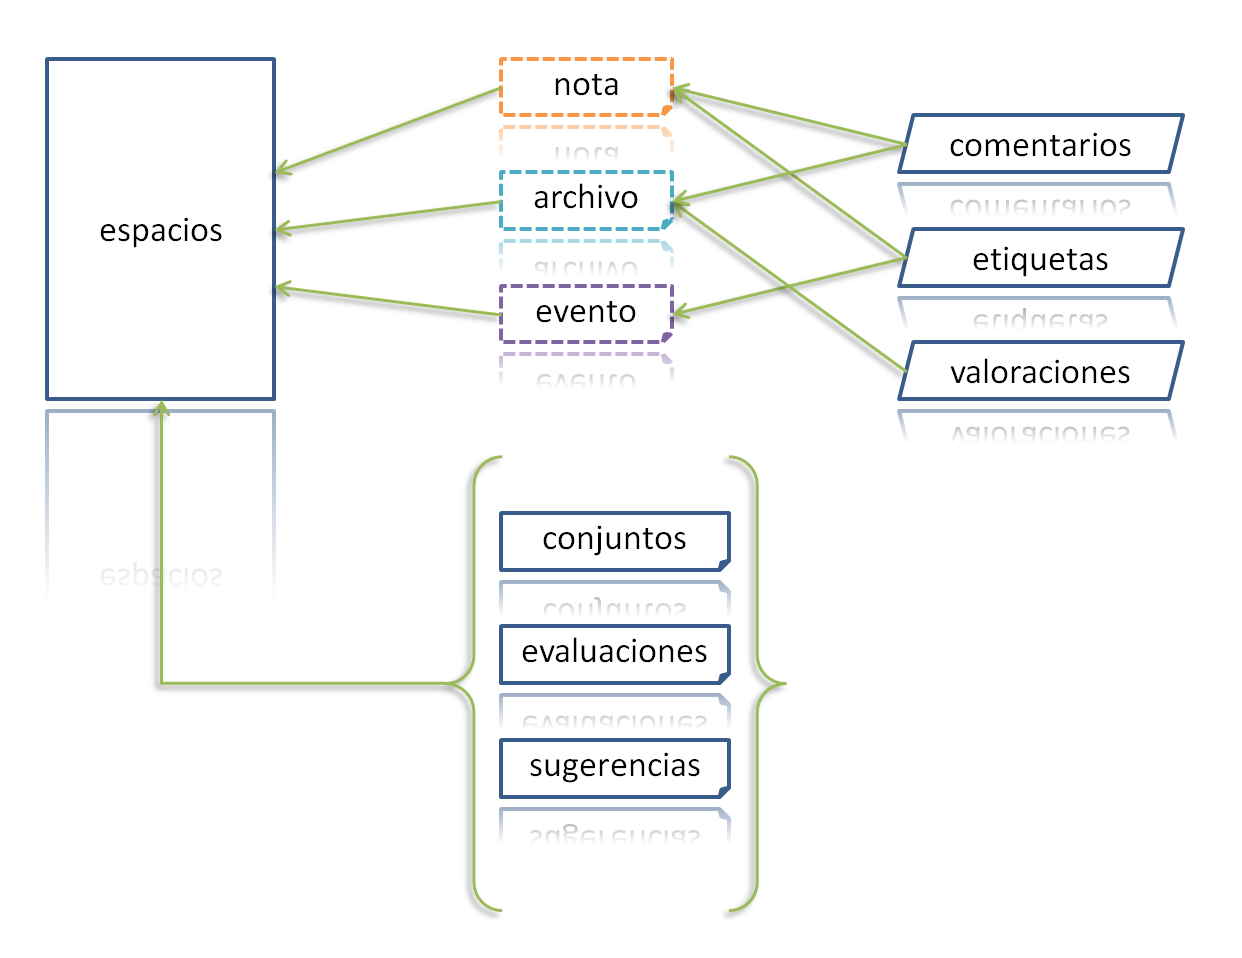
\includegraphics[scale=0.25]{graphics/nomenclatura.png}
 \caption {Relaci\'on entre los conceptos utilizados en el sistema}
 \label {nomenclatura}
\end{figure}

\subsection{Resultados}
Definidos los terminos a utilizarse, a continuaci\'on se present\'an los resultados generados:

\subsubsection{Contexto}
\begin{center}
\begin{tabular}{|l|l|}
\hline
Sitio web & \url{yachay.memi.umss.edu.bo} \\
Periodo acad\'emico & I/2011 \\
Tiempo de evaluaci\'on: & 325 dias. \\
Fecha de inicio: & 23 de Septiembre del 2010. \\
Fecha de fin: & 14 de Agosto del 2011. \\
Lugar de evaluaci\'on: & Carrera de Inform\'atica y Sistemas (UMSS). \\
Ca\'idas del servidor: & 4. \\
Tiempo del servidor fuera de linea: & 2 semanas acumuladas. \\
Docentes participantes: & 4. \\
Materias participantes: & 4. \\
Grupos participantes: & 8. \\
Usuarios participantes: & 542 (estudiantes de primeros semestres). \\
Espacios virtuales creados: & 33. \\
Recursos publicados: & 68. \\
\hline
\end{tabular}
\end{center}
\subsubsection{Usuarios}

En t\'erminos de uso, puede apreciarse en la Figura \ref{usuarios_tabla_1} las diferentes formas de comportamiento de los 
usuarios, seg\'un el rol que desempe\~nan en el sistema.
Destaca en esta tabla la disparidad entre el rol de estudiante y los dem\'as roles, como puede verse en la Figura 
\ref{usuarios_bars_1}, del conjunto de usuarios registrados, \'unicamente el 20\% ingreso alguna vez al sistema,
Es de rescatar adem\'as, que los usuarios fueron registrados autom\'aticamente por sus respectivos docentes.

\begin{figure}[H]
\centering
 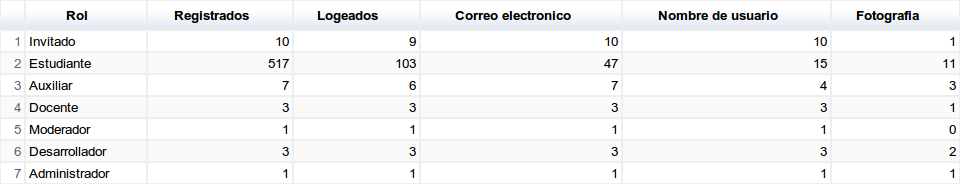
\includegraphics[scale=0.4]{graphics/usuarios_tabla_1.png}
 \caption {Intenci\'on de los usuarios clasificados por rol}
 \label {usuarios_tabla_1}
\end{figure}

\begin{figure}[H]
\centering
 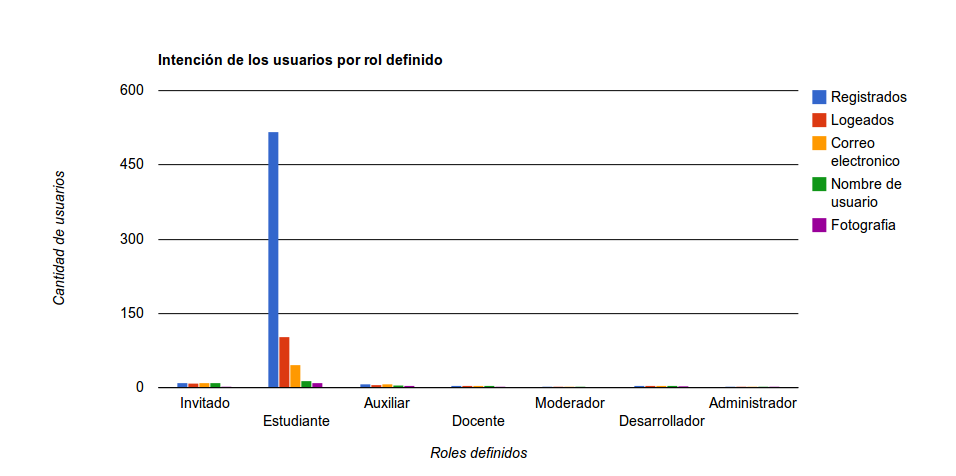
\includegraphics[scale=0.4]{graphics/usuarios_bars_1.png}
 \caption {Diagrama de barras de la intenci\'on de los usuarios clasificados por rol}
 \label {usuarios_bars_1}
\end{figure}

Puede verse en la Figura \ref{usuarios_pie_1} como el predominio en cantidad de los estudiantes va decayendo progresivamente
en intenci\'on frente a los otros roles. Considerando los escasa cantidad de atractivos que posee el sistema es importante 
considerar una audiencia de 126 personas como el primer paso hacia la construcci\'on de un lugar com\'un para el estudio 
realizado.\\

Respecto a la actividad de los usuarios sobre el sistema, puede verse en la Figura \ref{usuarios_tabla_2} la escasisima 
actividad, participaci\'on y popularidad en todos los roles, exceptuando el de los desarrolladores. Puede verse tambi\'en en
la Figura \ref{usuarios_bars_2} el prometedor indicador de sociabilidad, que como puede verse en la Figura 
\ref{usuarios_pie_2} es el mas homog\'eneo, lo que augura una conectividad mas que deseable para los usuarios.

\begin{figure}[H]
\centering
 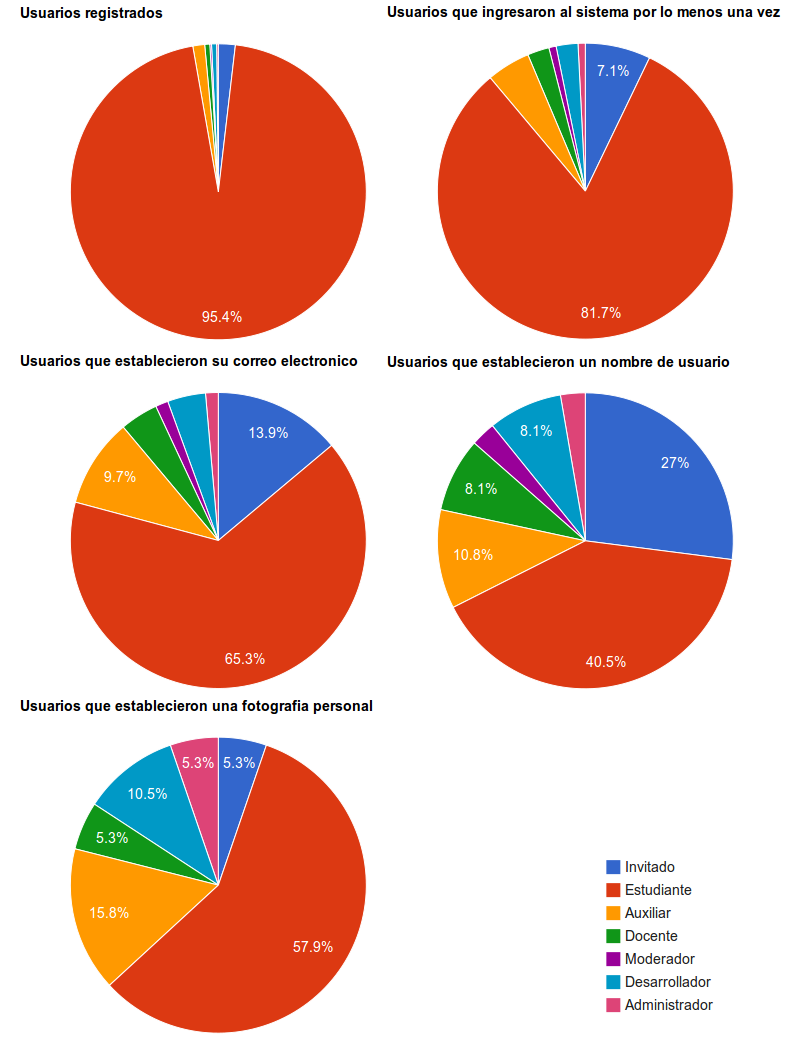
\includegraphics[scale=0.4]{graphics/usuarios_pie_1.png}
 \caption {Porcentajes de intenci\'on de los usuarios clasificados por rol}
 \label{usuarios_pie_1}
\end{figure}

\begin{figure}[H]
\centering
 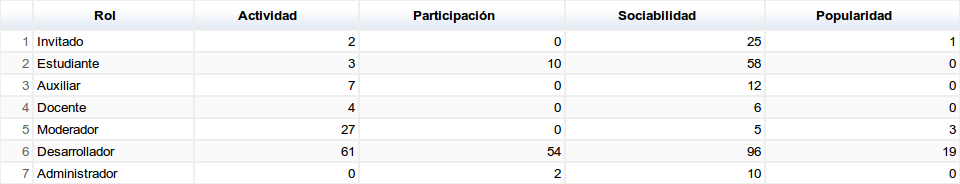
\includegraphics[scale=0.4]{graphics/usuarios_tabla_2.png}
 \caption {Actividad de los usuarios clasificados por rol}
 \label {usuarios_tabla_2}
\end{figure}

\begin{figure}[H]
\centering
 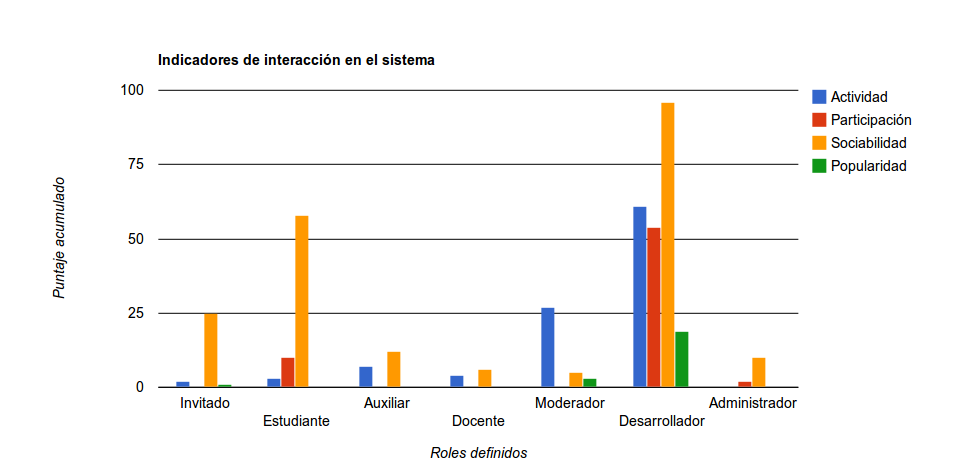
\includegraphics[scale=0.4]{graphics/usuarios_bars_2.png}
 \caption {Diagrama de barras de la actividad de los usuarios clasificados por rol}
 \label {usuarios_bars_2}
\end{figure}

\begin{figure}[H]
\centering
    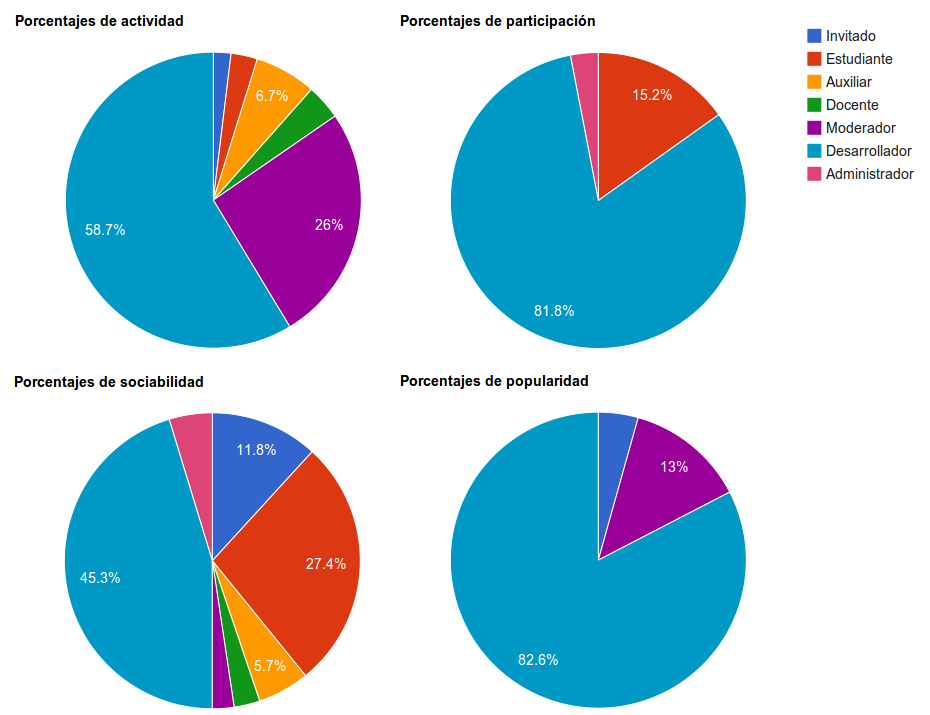
\includegraphics[scale=0.4]{graphics/usuarios_pie_2.png}
    \caption {Porcentajes de actividad clasificados por rol}
    \label {usuarios_pie_2}
\end{figure}

\subsubsection{Contactos}

Considerando los indicadores de sociabilidad, puede apreciarse la matriz de adyacencias (Figura \ref{contactos_matriz}) de la
red social, puede verse que los enlaces fuertes son casi exclusividad propia de los desarrolladores, siendo entre
los otros roles predominantes los enlaces d\'ebiles. Puede verse tambi\'en una sutil relaci\'on entre los usuarios que 
establecieron el nombre de usuario en su perfil, y los niveles de sociabilidad. Cuya interrelaci\'on, es motivo
de seguimiento e intenci\'on de demostraci\'on.
\begin{figure}[H]
\centering
    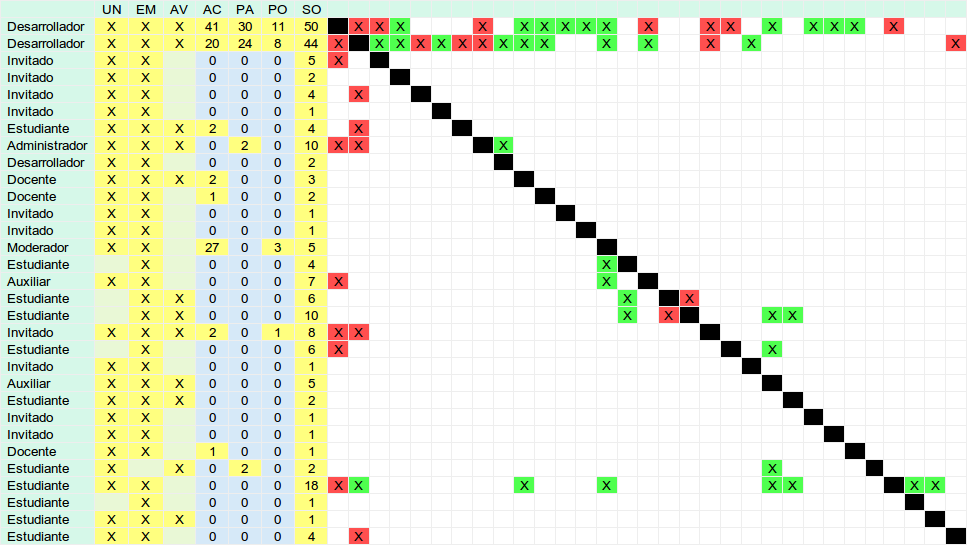
\includegraphics[scale=0.4]{graphics/contactos_matriz.png}
    \caption {Matriz de adyacencia de la red social}
    \label {contactos_matriz}
\end{figure}

\subsubsection{Espacios Virtuales}

En la Figura \ref{espacios_tabla_1} pueden verse los distintos tipos de espacios virtuales y sus indicadores propios, entre 
los que destaca la supremac\'ia del espacio portada, por sobre cualquier otro espacio, siendo el que 
capta mas audiencia de entre los espacios. Tambi\'en es notorio el ausente uso de espacios para equipos de trabajo en los 
grupos, cosa que puede ser debida a las escasez de grupos registrados. Si bien la portada acapara la 
mayor audiencia, no acapara la mayor cantidad de recursos (Figura \ref{espacios_bars_1}), llev\'andose los espacios de 
comunidades un 45\% del contenido del sitio, reforzando la teor\'ia de fomento hacia los espacios menos 
formales (Figura \ref{espacios_pie_1}).
\begin{figure}[H]
\centering
    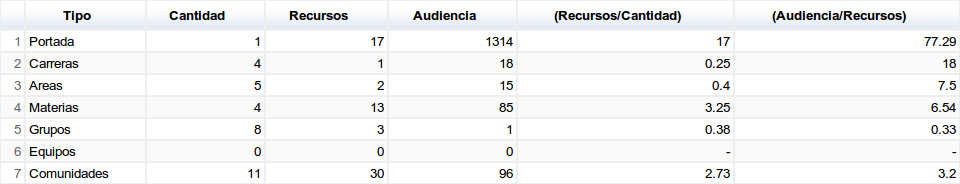
\includegraphics[scale=0.4]{graphics/espacios_tabla_1.png}
    \caption {Clasificaci\'on de los espacios y su actividad}
    \label {espacios_tabla_1}
\end{figure}

\begin{figure}[H]
\centering
    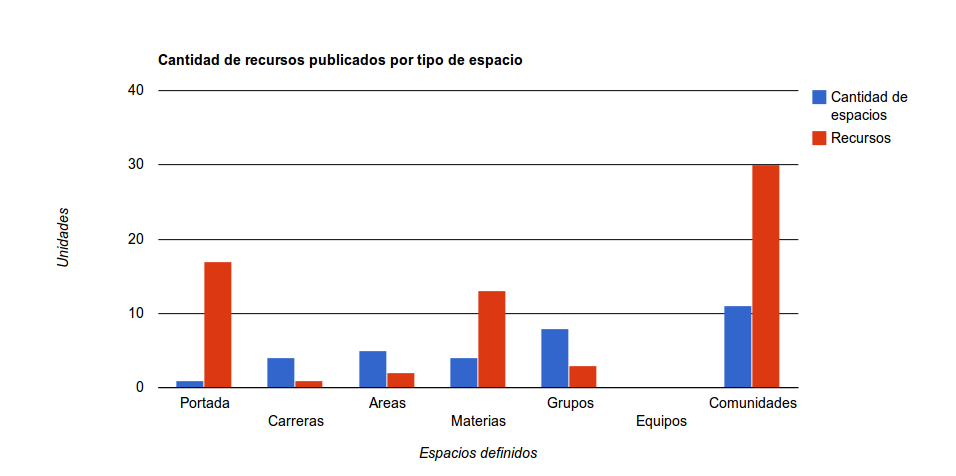
\includegraphics[scale=0.4]{graphics/espacios_bars_1.png}
    \caption {Diagrama de barras de los espacios y sus recursos}
    \label {espacios_bars_1}
\end{figure}

\begin{figure}[H]
\centering
    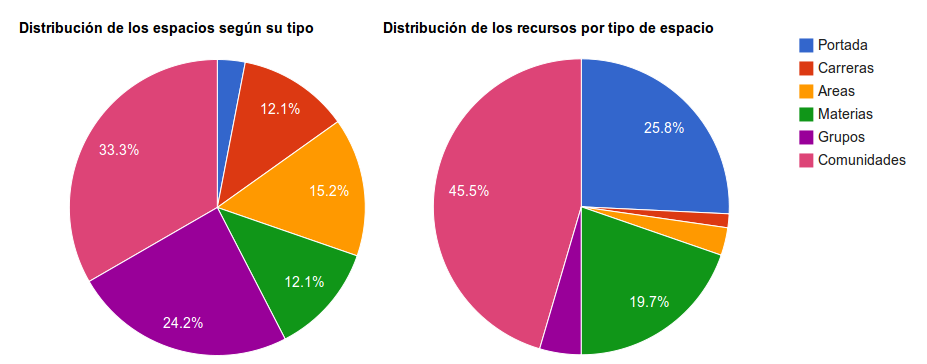
\includegraphics[scale=0.4]{graphics/espacios_pie_1.png}
    \caption {Porcentajes de los espacios y sus recursos seg\'un su tipo}
    \label {espacios_pie_1}
\end{figure}

\subsubsection{Recursos}

Los recursos pueden ser de varios tipos (Figura \ref{recursos_tabla_1}), destacando la gran cantidad de notas 
(Figura \ref{recursos_bars_1}) por sobre los otros tipos de recursos, pudiendo esto deberse a la inmensa facilidad de 
creaci\'on de estas. Aun asi son las fotograf\'ias la que en proporci\'on reciben mejor audiencia, y son los archivos los 
que reciben mayor cantidad de comentarios (Figura \ref{recursos_pie_1}).
\begin{figure}[H]
\centering
    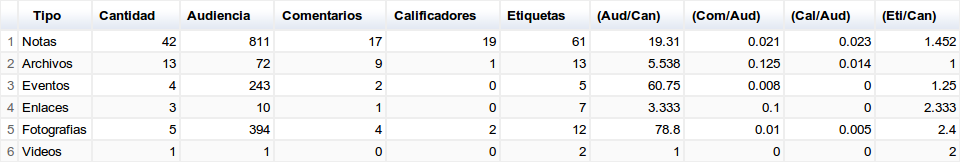
\includegraphics[scale=0.4]{graphics/recursos_tabla_1.png}
    \caption {Clasificaci\'on de los recursos seg\'un su tipo}
    \label {recursos_tabla_1}
\end{figure}

\begin{figure}[H]
\centering
    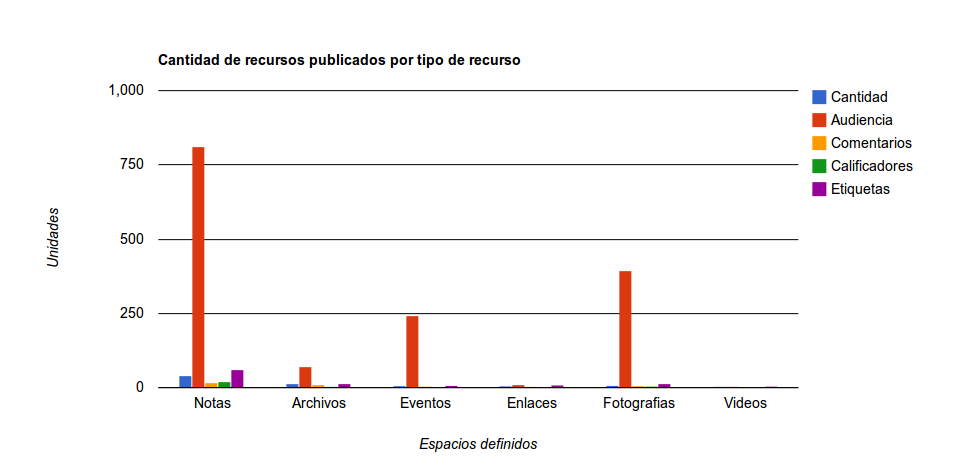
\includegraphics[scale=0.4]{graphics/recursos_bars_1.png}
    \caption {Diagrama de barras de los recursos y sus niveles de repercusi\'on}
    \label {recursos_bars_1}
\end{figure}

\begin{figure}[H]
\centering
    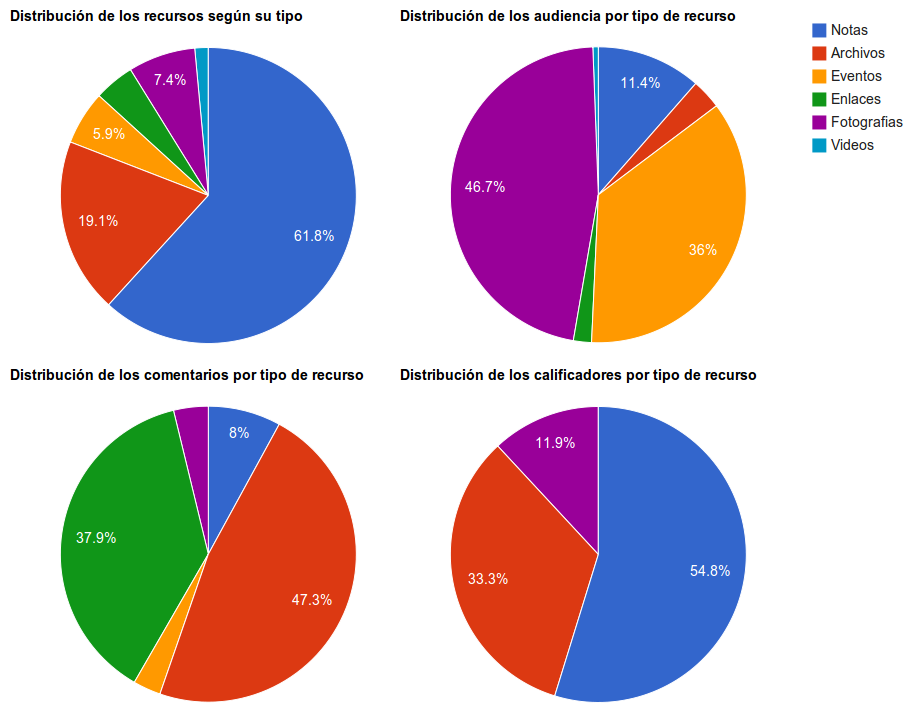
\includegraphics[scale=0.4]{graphics/recursos_pie_1.png}
    \caption {Porcentajes de los recursos seg\'un su tipo}
    \label {recursos_pie_1}
\end{figure}

\subsubsection{Linea de tiempo}

Finalizados los elementos propios de la herramienta, se observan ahora las lineas de tiempo, donde se presentan los tiempos
en los que estos elementos han sido creados.
En la Figura \ref{tiempos_area_1} puede apreciarse en la linea de creaci\'on de los usuarios, los registros autom\'aticos de 
los estudiantes, de parte del docente de su materia, siendo la creaci\'on de usuarios la linea predominante en esta gr\'afica.
\begin{figure}[H]
    \centering
    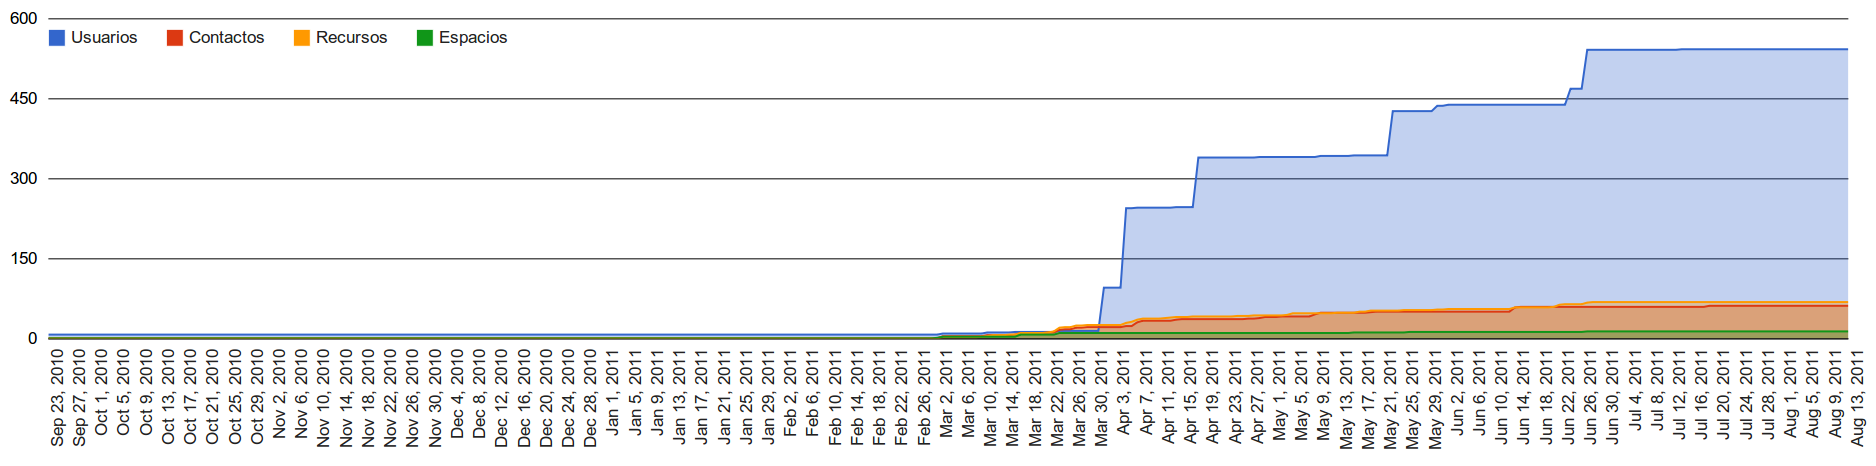
\includegraphics[scale=0.25]{graphics/tiempos_area_1.png}
    \caption {Linea de tiempo de la creaci\'on de elementos en el sistema}
    \label {tiempos_area_1}
\end{figure}

En la Figura \ref{tiempos_area_2} resalta la curiosa relaci\'on entre las lineas de creaci\'on de recursos y la de creaci\'on
de contactos, siendo esta la linea que determina todo el objeto de investigaci\'on.
\begin{figure}[H]
\centering
    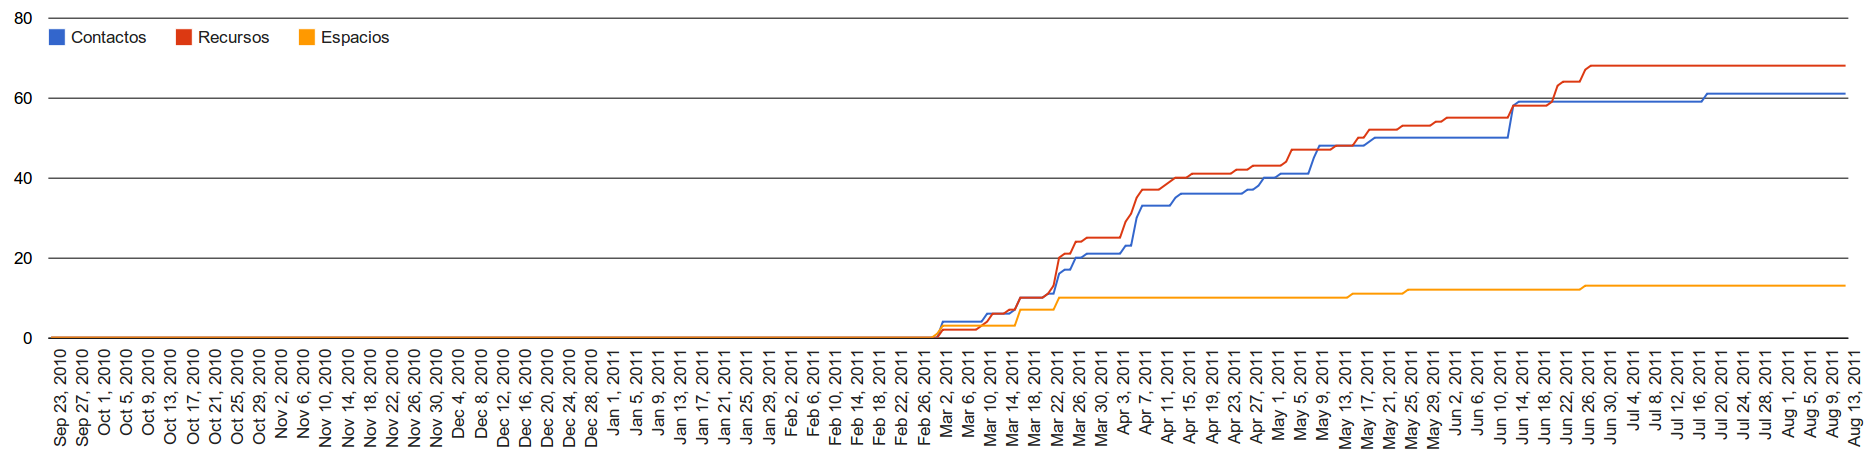
\includegraphics[scale=0.25]{graphics/tiempos_area_2.png}
    \caption {Linea de tiempo de la creaci\'on de elementos en el sistema}
    \label {tiempos_area_2}
\end{figure}

\newpage
\begin{thebibliography}{99}
 \bibitem{Conetivismo} \textsc{George Siemens.:}
              \textit{\textbf{Conectivismo: Una teor\'ia de aprendizaje para la era digital.}}
              \par Diciembre 12, 2004.

 \bibitem{tdl} \textsc{George Siemens.:}
            \textit{\textbf{The value of diversity in learning.}}
            \par \url{http://www.connectivism.ca/?p=24}

 \bibitem{as} \textsc{Andres Schuschny.:}
             \textit{\textbf{Conectivismo: una teor\'ia del aprendizaje para la era digital.}}
             \par \url{http://humanismoyconectividad.wordpress.com/2009/01/14/conectivismo-siemens/}

 \bibitem{social} \textsc{\textbf{The Social Learning Theory of Julian B. Rotter}}
                 \par \url{http://psych.fullerton.edu/jmearns/rotter.htm}
 
 \bibitem{diapositiva} \textsc{Fernando Luna Pizarro Quinteros.:}
                       \textsc{\textbf{Estrategias de aprendizaje 2.0 - enfoque te\'orico}}

 \bibitem{web} \textsc{James Governor, Dion HinchclifFe, Duane Nickull.:}
               \textsc{\textbf{ Web 2.0 Architectures.}}
               \par O'Reilly
                                       
 \bibitem{web2.0} \textsc{Crist\'obal Cobo Roman\'i, Hugo Pardo Kuklinski.:}
                  \textsc{\textbf{Planeta Web 2.0 inteligencia colectiva o medio fast food}}
                  \par \url{http://www.planetaweb2.net/}                   
%  \bibitem{blog} \textsc{\textbf{Blog oficial de George Siemens.}}
% 		\par \url{http://www.connectivism.ca}   

 \bibitem{Tam} \textsc{Sandra L. CastilloVallejo.:}
               \textit{\textbf{Teor\'ia de la actividad:Una perspectiva en la ense\~nanza de la matem\'atica apoyada en el
                               uso de las tecnolog\'ias de informaci\'on y comunicaci\'on}}
               \par Diciembre 6, 2007.
  

\end{thebibliography}

\newpage
\begin{figure}
 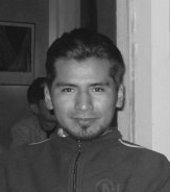
\includegraphics[scale=0.5]{graphics/antonio.png}
\end{figure}
\textbf{Antonio Mamani}\\
Estudiante de Lic. en Inform\'atica en la Universidad Mayor de San Sim\'on que realiz\'o el curso de Apply Functional Programming 
en la Universidad de Utrecht, Holanda. Asistente de investigaci\'on del centro MEMI-UMSS. Miembro de la comunidad Haskell 
San Sim\'on. Ex-competidor del concurso ACM-ICPC. Co-organizador y capacitador de estudiantes de la UMSS para las 
competencias ACM-ICPC-Bolivia. 

\end{document}
